\section{Distribution Analysis}
\label{sec:dist}

\begin{figure}[t!]
\begin{center}
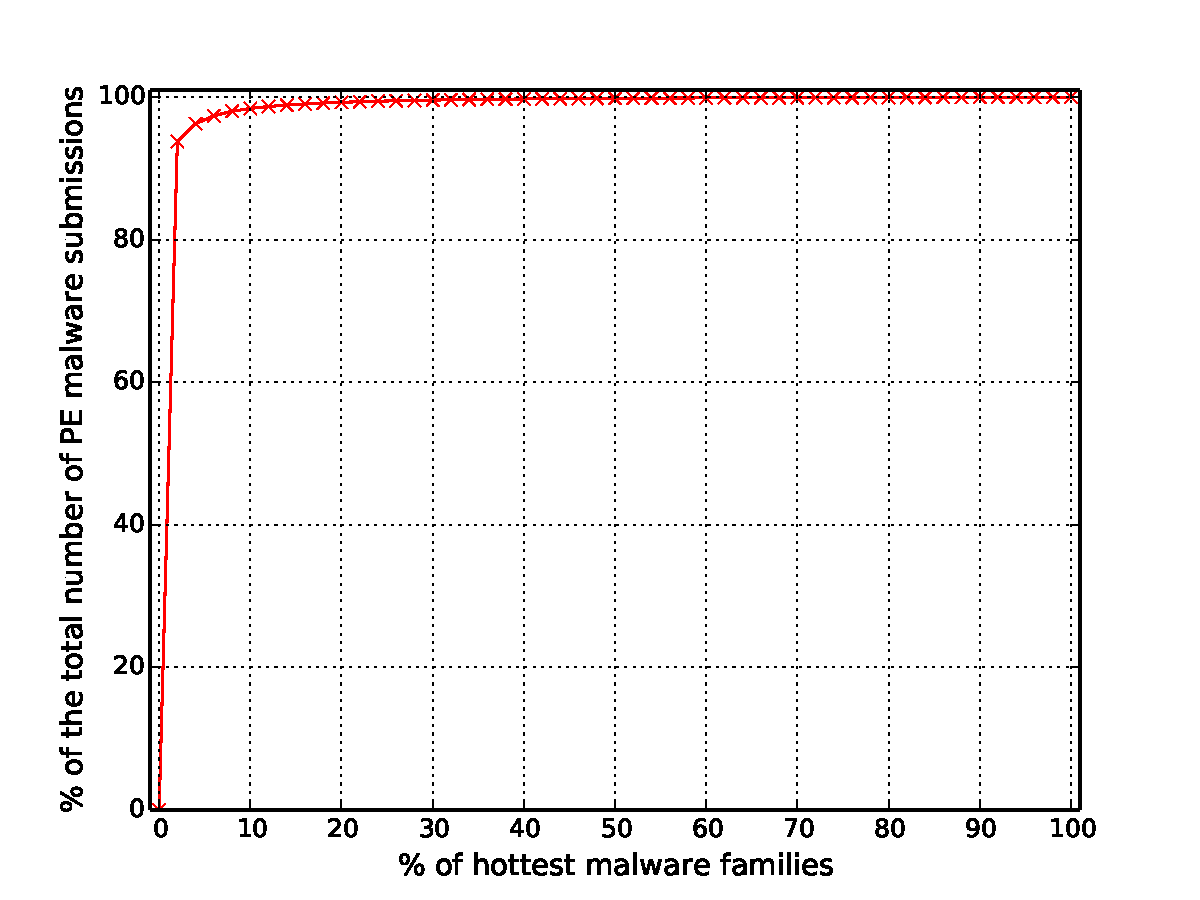
\includegraphics[width=2.5in]{figure/cum}
\caption{Skewness of malware families appearing in November of 2015.}
\label{fig:acum}
\end{center}
\end{figure}

\begin{figure*}[!htb]
\minipage{0.22\textwidth}
  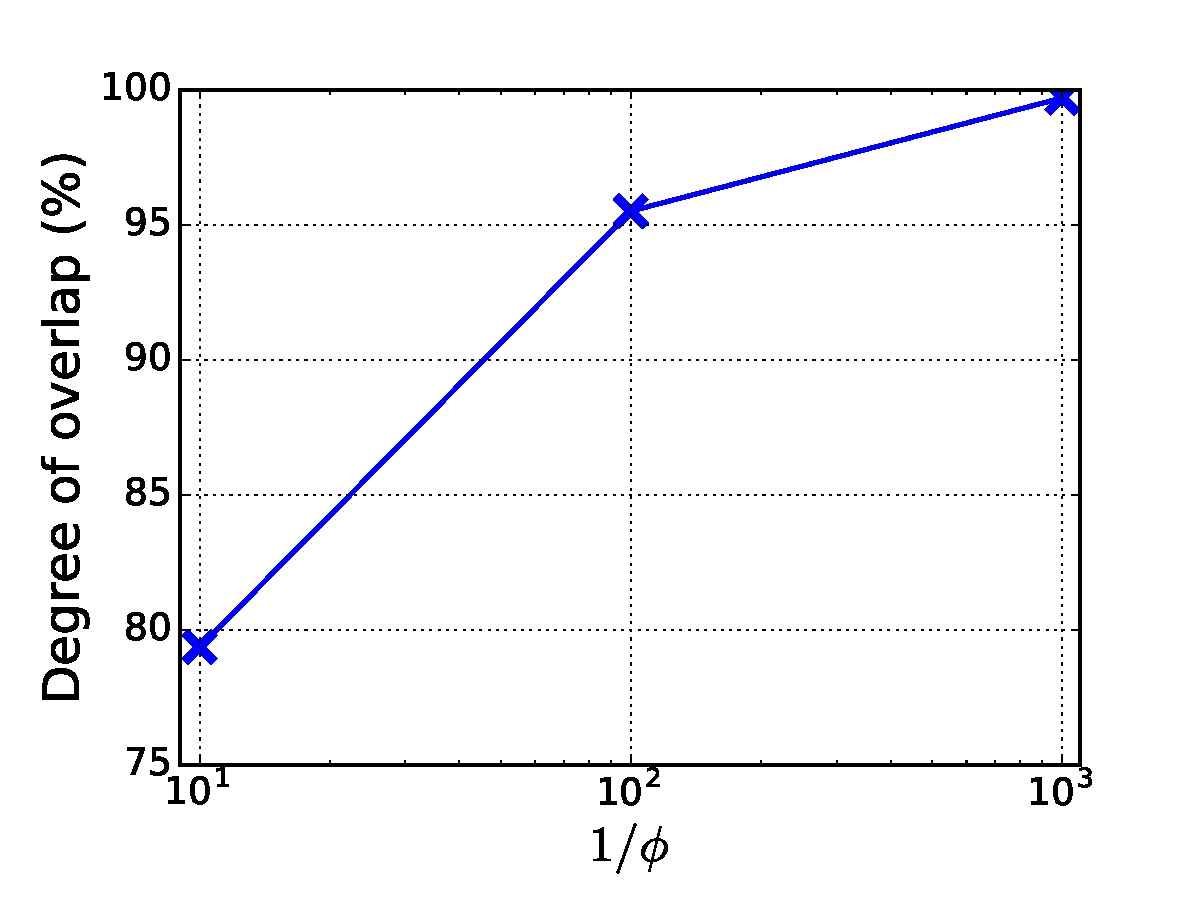
\includegraphics[width=\linewidth]{figure/overlap.pdf}
  \caption{Relation between $\phi$ and degree of overlap.}
  \label{fig:overlap}
\endminipage\hfill
\minipage{0.22\textwidth}
  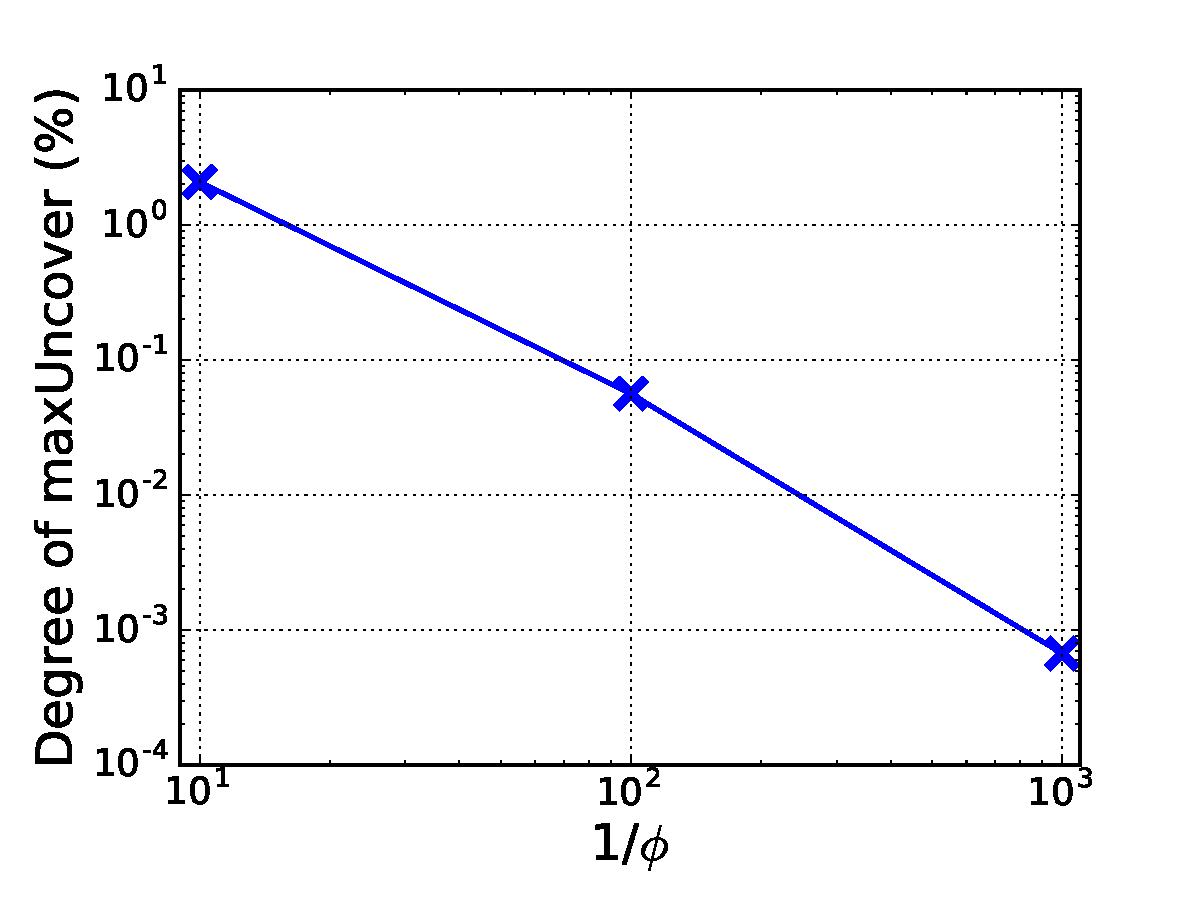
\includegraphics[width=\linewidth]{figure/maxUncover.pdf}
  \caption{Relation between $\phi$ and degree of maxUncover.}
  \label{fig:maxUncover}
\endminipage\hfill
\minipage{0.22\textwidth}%
  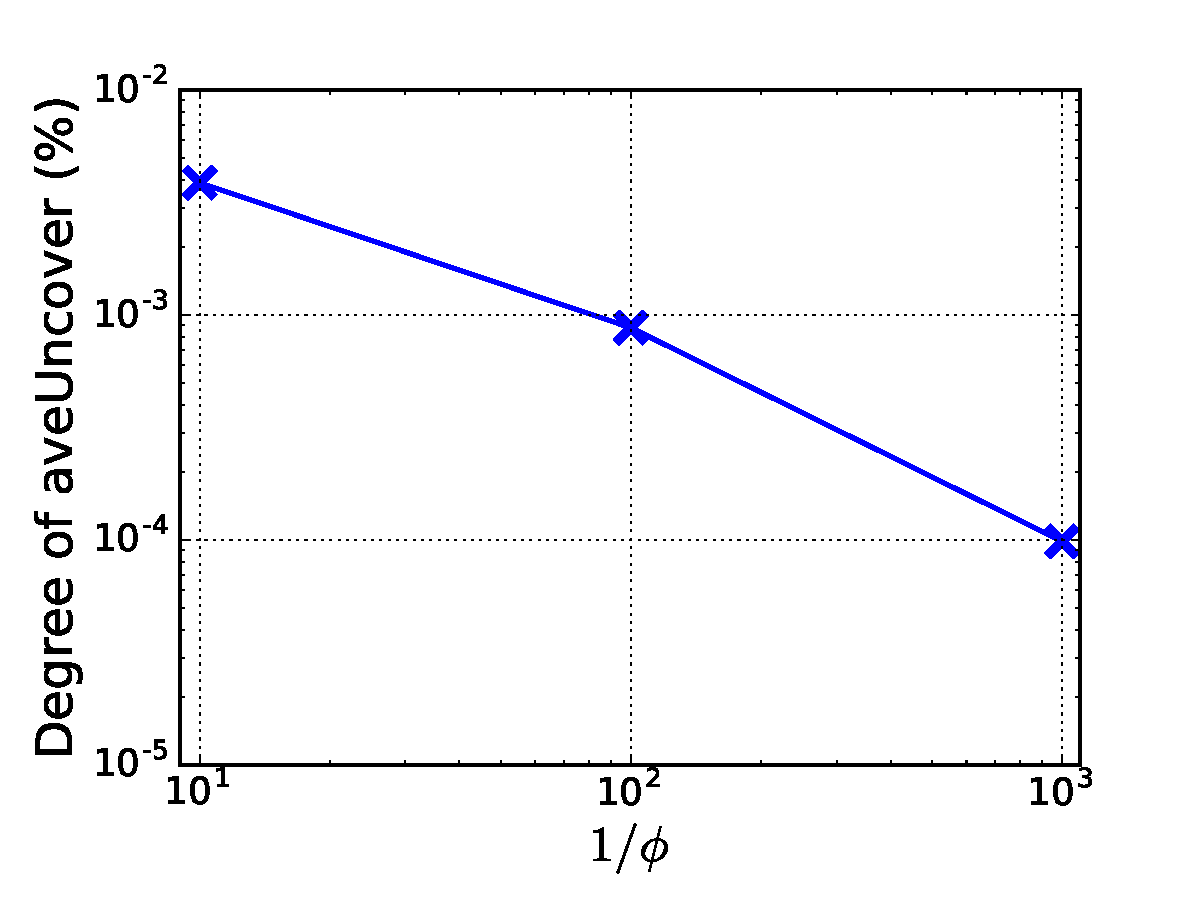
\includegraphics[width=\linewidth]{figure/aveUncover.pdf}
  \caption{Relation between $\phi$ and degree of aveUncover.}
  \label{fig:aveUncover}
\endminipage\hfill
\minipage{0.22\textwidth}%
  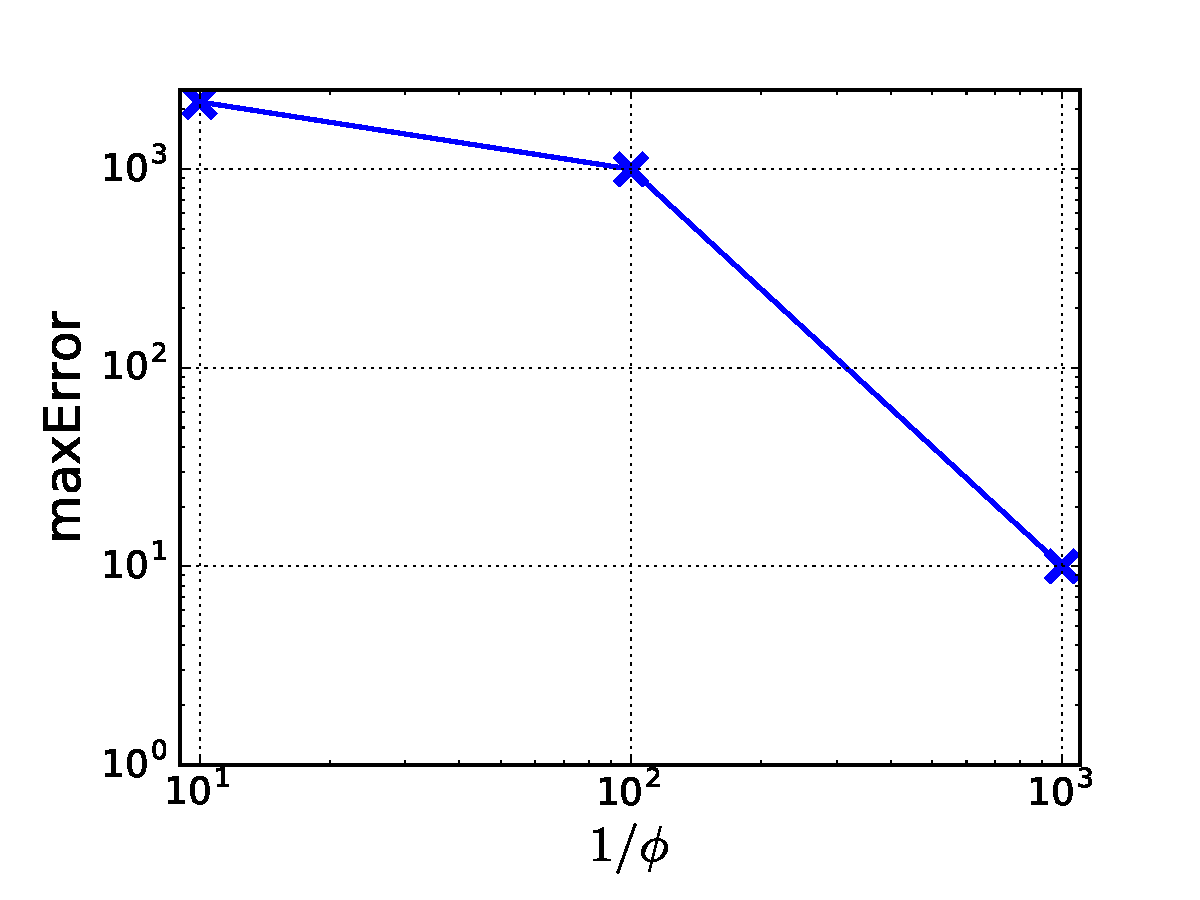
\includegraphics[width=\linewidth]{figure/maxError.pdf}
  \caption{Relation between $\phi$ and maxError.}
  \label{fig:maxError}

\endminipage
\end{figure*}

\begin{figure}[t!]
\begin{center}
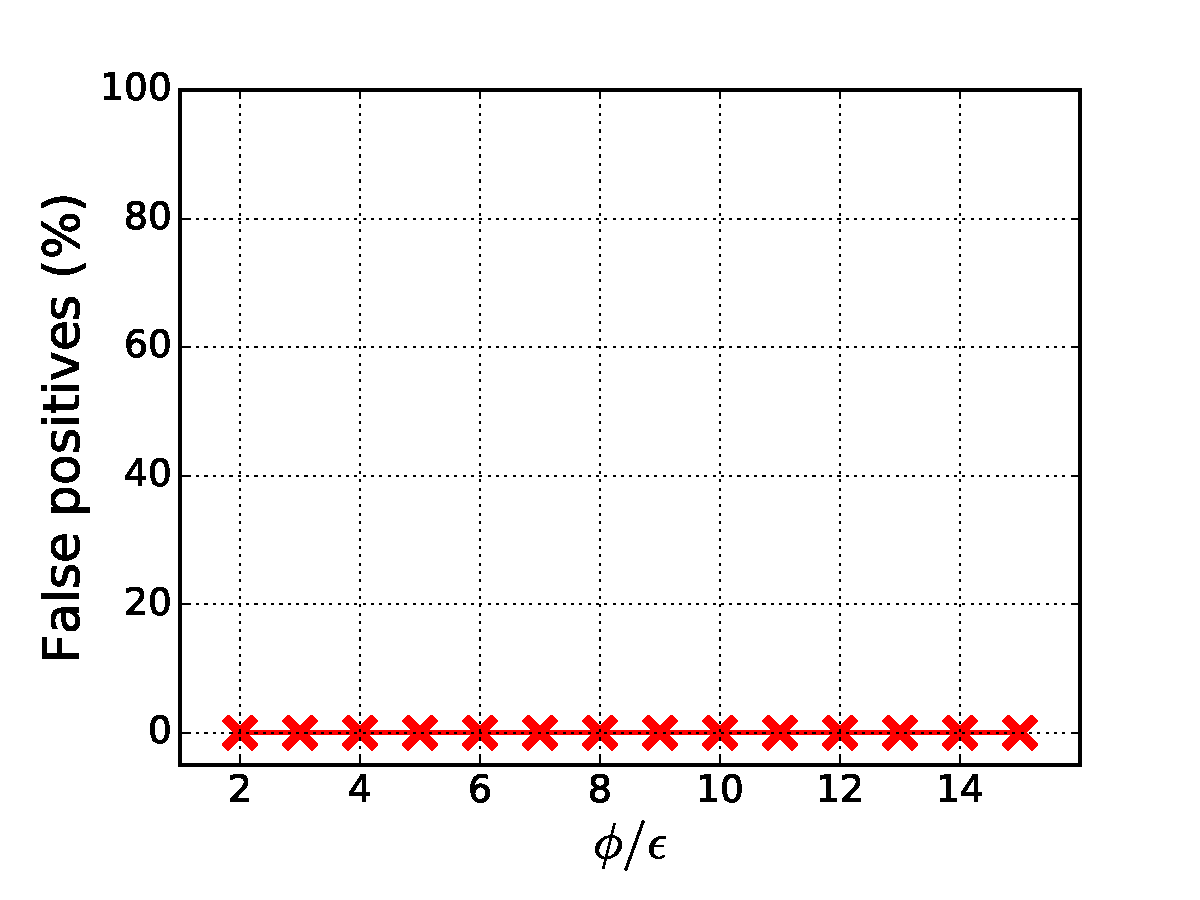
\includegraphics[width=2.0in]{figure/fp}
\caption{False positives in $(\phi, \epsilon)\mbox{-}HMF$ as a function of $\epsilon$. The value of $\phi$ is fixed to $10^{-2}$.}
\label{fig:fp}
\end{center}
\end{figure}


In this section, we study how malwares distributed in each malware family. 

As shown in Figure~\ref{fig:acum}, only small number of malware families are hot.
The distribution of malware families follows the well-known Pareto principle, 
and more than 90\% malware families take place in only 10\% malwares. 

{\bf Observation 3:} the distribution of malware families is highly skewed. 




The skewness of malware families indicates we could apply frequent item mining algorithm to identify hot malware families. 

Frequent item mining algorithms take two configuration parameters, $\phi$ and $\epsilon$, where $\phi > \epsilon$. 
The goal of frequent item mining algorithms are to provide nearly-real time analysis on massive data streams by using constant memory. 
Assuming the length of the input stream is $N$, the output of frequent item mining algorithms 
are all items which appear more than $\lfloor \phi N \rfloor$ times, 
and no items which appear less than  $\lfloor \epsilon N \rfloor$ times. 


The frequent item mining algorithm we use is space saving algorithm~\cite{space-saving}, 
which was proposed for streams in Internet advertising, and has already been applied in other areas, 
like mining hot calling contexts in profilers~\cite{hot-calling-context}.
Space saving algorithm tracks $M=1/\epsilon$ pairs of $(f, c)$. 
$f$ is short for malware family, and $c$ is short for counter.  
Content of these pairs represents $(\phi, \epsilon)\mbox{-}HMF$ (Hot Malware Family). 
The $M$ pairs are initialized with the first $M$ encountered malware families and their frequency. 
When a new malware submission comes, 
if the malware family is already under monitoring, 
the related counter will be increased by 1. 
And if the malware family is not monitored, 
we will replace the malware family of the pair with lowest counter value with the incoming malware family, 
and increase its counter value by 1. 
When querying HMF, 
all malware families whose counter values are larger than $\lfloor \phi N \rfloor$ will be returned. 




We implement the space saving algorithm by using python-2.7, 
and conduct experiments in the same system as we did in Section~\ref{sec:temporal}.
Following previous works in frequent item mining~\cite{hot-calling-context}, 
we measure the following metrics by using malware submission data we collect:

\begin{enumerate}

\item 
Degree of \textit{overlap} is used to measure the percentage of malwares covered in $(\phi, \epsilon)\mbox{-}HMF$,
and it is defined as follows:

\begingroup\makeatletter\def\f@size{8}\check@mathfonts
$$overlap((\phi, \epsilon)\mbox{-}HMF) = \dfrac{1}{N}\sum_{f \in (\phi, \epsilon)\mbox{-}HMF}w(f)$$
\endgroup

where $w(f)$ represents the real frequency of malware family $f$.  

\item 
\textit{MaxUncover} is short for maximum frequency of uncovered malware families. 
%is used 
%to measure largest frequency of malware families not covered in $(\phi, \epsilon)\mbox{-}HMF$. 
It is defined as follows:
\begingroup\makeatletter\def\f@size{8}\check@mathfonts
$$maxUncover((\phi, \epsilon)\mbox{-}HMF) = \max_{f \notin (\phi, \epsilon)\mbox{-}HMF}w(f)/H(f)$$
\endgroup
where $H(f)$ is the maximum frequency of all malware families. 

\item 
\textit{AveUncover} is short for average frequency of uncovered malware families 
and it is defined similar to \textit{maxUncover}. 

\item 
\textit{False positives} are defined as malware families returned when querying HMF, 
but whose real frequencies are less than $\lfloor \phi N \rfloor$. 
Space saving algorithm is designed to guarantee that there will be no false negatives. 

\item 
\textit{MaxError} is used to measure relative error of counter values, 
compared with their real frequencies.
It is defined as follows:
\begingroup\makeatletter\def\f@size{8}\check@mathfonts
$$maxError((\phi, \epsilon)\mbox{-}HMF) = \max_{f \in (\phi, \epsilon)\mbox{-}HMF} \dfrac{\left|c(f) - w(f)\right|}{w(f)}$$
\endgroup

\end{enumerate}

There are two configuration parameters in space saving algorithm: $\phi$ and $\epsilon$, 
and the number of monitored $(f, c)$ pairs is directly controlled by $\epsilon$. 
Following previous experience of applying space saving algorithm~\cite{hot-calling-context}, 
we set $\epsilon = \phi/5$ as default, 
unless we explicitly state.  

We first evaluate how the degree of \textit{overlap} would change with the change of $\phi$. 
The degree of \textit{overlap} is used to describe how many malwares are monitored in $(\phi, \epsilon)\mbox{-}HMF$, and it is the larger the better. 
As shown by Figure~\ref{fig:overlap}, after we change $\phi$ from 10 to 100, the degree of \textit{overlap} will increase from 79.93\% to 95.48\%. 
The degree of \textit{overlap} will further increase to 99.70\%, after we change $\phi$ to 1000. 

We then study how maxUncover and aveUncover would change with the change of $\phi$.
Both maxUncover and aveUncover are used to describe malwares not monitored in $(\phi, \epsilon)\mbox{-}HMF$, 
and they are the lower the better. As shown by Figure~\ref{fig:maxUncover} and Figure~\ref{fig:aveUncover}, 
both maxUncover and aveUncover will decrease by an order, as we increase $\phi$ value by an order. 

Figure~\ref{fig:maxError} shows how \textit{maxError} change, after we change $\phi$. 
\textit{maxError} describes how precise counters in $(\phi, \epsilon)\mbox{-}HMF$ are, 
and it is the lower the better. \textit{maxError} would drop from 2178 to 999, 
after we change the value of $\phi$ from 10 to 100. 
\textit{maxError} value would become to 10, after we change the value $\phi$ to 1000. 
The large \textit{maxError} value is due to the fact that space saving algorithm 
will conservatively assume the frequency of a new malware family is one larger than the least counter value of all monitored malware family. 

In the last experiment, we fix $\phi$ to $10^{-2}$, 
and change $\phi/\epsilon$ from 2 to 15 to evaluate how false positives would change. 
As shown by Figure~\ref{fig:fp}, space saving algorithm will constantly report 0 false positives in our experiments. 

\underline{Discussion.}
Distributions of malware families are highly skewed. 
This is the reason why we could precisely identify hot malware families. 
There are in total 11311 distinct malware families in our tested data. 
Although this number is small, new malware families would appear every day, 
and applying frequent item mining algorithm can identify hot malware families from possibly 
infinite malware families by only using constant memory. 

As we discussed in Section~\ref{sec:temporal}, malware family is a relative coarse granularity.
In the future, we could consider how to mining frequent items in a finer granularity. 